\documentclass[pdflatex,sn-vancouver-num]{sn-jnl}

\usepackage{graphicx}%
\usepackage{multirow}%
\usepackage{amsmath,amssymb,amsfonts}%
\usepackage{amsthm}%
\usepackage{mathrsfs}%
\usepackage[title]{appendix}%
\usepackage{xcolor}%
\usepackage{textcomp}%
\usepackage{manyfoot}%
\usepackage{booktabs}%
\usepackage{algorithm}%
\usepackage{algorithmicx}%
\usepackage{algpseudocode}%

\theoremstyle{thmstyleone}%
\newtheorem{theorem}{Theorem}%
\newtheorem{proposition}[theorem]{Proposition}%
\newtheorem{lemma}[theorem]{Lemma}%
\newtheorem{corollary}[theorem]{Corollary}%
\theoremstyle{thmstyletwo}%
\newtheorem{example}{Example}%
\newtheorem{remark}{Remark}%
\theoremstyle{thmstylethree}%
\newtheorem{definition}{Definition}%
\newtheorem{problem}{Problem}%

\newcommand{\DB}{\mathcal{D}}
\newcommand{\pr}{\mathit{pr}}
\newcommand{\qty}{q}
\newcommand{\prob}{p}
\newcommand{\uu}{u}
\newcommand{\EU}{\mathit{EU}}
\newcommand{\EP}{\mathit{EP}}
\newcommand{\PTU}{\mathit{PTU}}
\newcommand{\PTWU}{\mathit{PTWU}}
\newcommand{\PUB}{\mathit{PUB}}
\newcommand{\rem}{\mathit{rem}}
\newcommand{\minprob}{\mathit{minProb}}
\newcommand{\itemset}{X}

\raggedbottom

\begin{document}

\title[Parallel Top-K PPNHUI Mining]{Parallel Methods for Mining Top-$K$ Probabilistic Positive--Negative High-Utility Itemsets from Uncertain Databases: A Shared-Memory Design-Space Study}

\author[1,2]{\fnm{Huy} \sur{Vo}}
\author[1,2]{\fnm{Nguyen} \sur{Le}}
\equalcont{These authors contributed equally to this work.}
\author*[2]{\fnm{Thien} \sur{Nguyen}}\email{nguyenchithien@tdtu.edu.vn}
\equalcont{These authors contributed equally to this work.}
\affil[1]{\orgdiv{Faculty of Information Technology}, \orgname{Ton Duc Thang University}, \orgaddress{\city{Ho Chi Minh City}, \country{Vietnam}}}
\affil[2]{\orgdiv{Natural Language Processing and Knowledge Discovery Laboratory, Faculty of Information Technology}, \orgname{Ton Duc Thang University}, \orgaddress{\city{Ho Chi Minh City}, \country{Vietnam}}}

\abstract{%
Top-$K$ high-utility itemset mining frees the analyst from choosing a minimum
utility threshold, mining over \emph{uncertain} databases models the existence
probabilities that arise from noisy or aggregated data, and admitting
\emph{negative} item profits captures losses that co-occur with gains. Combining
all three yields the Top-$K$ Probabilistic Positive--Negative High-Utility
Itemset (PPNHUI) problem, whose enlarged search space makes parallel execution
attractive. Yet the \emph{effectiveness} of parallelism is not obvious: the
top-$K$ admission threshold only rises as high-utility itemsets are found, and
how quickly it rises depends on the data. This paper presents a shared-memory
design-space study. We define a common mining core based on a
utility--probability list (UPU-List) with a three-tier ($\EP$, $\PTWU$, $\PUB$)
pruning scheme, prove that all three tiers remain valid upper bounds when item
profits may be negative, and instantiate the core under five parallelisation
strategies spanning two design axes: threshold sharing (global vs.\ thread-local)
and load balancing (static, dynamic, work-stealing). Using a \emph{work-ratio}
metric (joins performed relative to the sequential baseline) we separate
algorithmic effects from raw hardware parallelism. Experiments on four datasets
reveal a clear regime spectrum: on dense data (Chess, Mushroom) cooperative
threshold escalation lets the work-stealing strategy do as little as one tenth
of the sequential work and reach up to $27.5\times$ speedup on eight cores
(super-linear), whereas on sparse retail data (Liquor, Retail) the same strategy
performs more work than the baseline and a producer--consumer strategy is the
most robust. The non-sharing strategy is consistently the worst and can run
slower than sequential. The work-ratio metric explains the entire spectrum and
identifies which parallel strategy to prefer for a given regime.
}

\keywords{high-utility itemset mining, uncertain databases, top-$k$ mining,
negative utility, parallel algorithms, shared-memory parallelism}

\maketitle

\section{Introduction}\label{sec:intro}
High-utility itemset mining (HUIM) generalises frequent itemset mining by
weighting items with utilities such as profit, revealing patterns that are
valuable rather than merely frequent~\cite{liu2012huiminer,gan2021survey}. Three
extensions move HUIM closer to real applications. First, the analyst rarely
knows a good minimum-utility threshold; \emph{top-$K$} mining instead asks
directly for the $K$ itemsets of highest utility~\cite{wu2012topk,tseng2016topk}.
Second, data gathered from sensors, imputation, or aggregation is
\emph{uncertain}: each item in a transaction carries an existence
probability~\cite{lin2016phuim}. Third, real profit tables contain
\emph{negative} entries---loss leaders, penalties, adverse events---so a faithful
model must allow items with negative utility~\cite{chu2009huiniv,lin2016fhn}.

Combining all three yields the Top-$K$ Probabilistic Positive--Negative
High-Utility Itemset (PPNHUI) problem. Negative items prevent the search from
being pruned by utility alone and so enlarge it, which motivates parallel
execution. However, whether parallelism actually helps is subtle. Top-$K$
algorithms prune using an admission threshold that equals the $K$-th best utility
found \emph{so far}; this threshold starts low and rises only as good itemsets
are discovered~\cite{tseng2016topk}. In a parallel execution many branches are
explored before the threshold has risen, creating redundant work; conversely, if
several workers \emph{share} the threshold, an early discovery by one worker can
prune the others. Which effect dominates is data-dependent, and negative items,
by depressing utilities, slow the threshold's ascent. A study of parallel PPNHUI
mining therefore needs a metric that separates algorithmic pruning from raw
hardware speedup.

This paper provides such a study for the \emph{shared-memory} setting, where the
exact, instantaneous sharing of a global threshold is possible---something a
distributed engine cannot easily offer. Our contributions are:
\begin{enumerate}
\item We formalise the Top-$K$ PPNHUI problem over uncertain databases
      (Section~\ref{sec:prelim}) and a common mining core built on a
      utility--probability list (UPU-List) with a three-tier
      ($\EP$, $\PTWU$, $\PUB$) pruning scheme (Section~\ref{sec:methods}).
\item We prove that all three pruning tiers remain valid upper bounds when item
      profits may be negative and that the resulting search is exact
      (Lemmas~\ref{lem:ep}--\ref{lem:pub}, Theorem~\ref{thm:correct}).
\item We instantiate the core under five shared-memory parallel strategies that
      span two design axes---threshold sharing and load balancing---and analyse
      them with a \emph{work-ratio} metric.
\item On four datasets we show a regime spectrum: cooperative threshold
      escalation yields up to $27.5\times$ (super-linear) speedup on dense data
      but degrades on sparse data, where a producer--consumer strategy is most
      robust; the non-sharing strategy is always worst and can be slower than
      sequential (Sections~\ref{sec:results}--\ref{sec:discussion}).
\end{enumerate}

\section{Related Work}\label{sec:related}
\paragraph{Top-$K$ HUIM.}
Top-$K$ HUIM removes the minimum-utility threshold. Two-phase methods such as
TKU~\cite{wu2012topk} and REPT~\cite{ryang2015rept} first generate candidates and
then verify them, while one-phase methods such as TKO~\cite{tseng2016topk} and
KHMC~\cite{duong2016khmc} use a vertical utility-list~\cite{liu2012huiminer} and
raise the threshold during a single traversal. All of these target
\emph{certain} databases with non-negative utilities.

\paragraph{HUIM over uncertain databases.}
Lin et al.~\cite{lin2016phuim} introduced potential high-utility itemset mining
(PHUIM) for uncertain data, with the level-wise PHUI-UP and the list-based
PHUI-List built on a probability-utility (PU) list; MUHUI~\cite{lin2017muhui}
adds pruning to the same structure. These methods mine \emph{all} potential
high-utility itemsets rather than a top-$K$ set, and assume non-negative profits.

\paragraph{HUIM with negative utilities.}
HUINIV-Mine~\cite{chu2009huiniv} first handled negative item values;
FHN~\cite{lin2016fhn} introduced a positive-and-negative utility list (PNU-list)
that is far faster, and surveys document the area~\cite{singh2018negsurvey}. Most
recently, TopHUI~\cite{gan2020tophui} performs \emph{top-$K$} HUIM with negative
utility---but for \emph{certain} databases. Our UPU-List combines the PU-list
idea of~\cite{lin2016phuim} with the positive/negative bookkeeping
of~\cite{lin2016fhn}; the structure itself is therefore evolutionary rather than
novel, which is why our contribution is the parallel study, not the data
structure.

\paragraph{Parallel and distributed HUIM.}
Big-data HUIM has largely been distributed: PHUI-Growth on
Hadoop~\cite{lin2015bigdata}, PKU for parallel top-$K$ HUIM on
Spark~\cite{lin2019pku}, P-FHM+ on Spark~\cite{sethi2018pfhm}, and GPU-based
heuristics~\cite{fang2024gpu}. These frameworks partition the work into largely
independent subtasks and therefore cannot share an exact global threshold across
nodes. Shared-memory multi-core HUIM has received far less attention, and to our
knowledge no prior work studies how the choice of shared-memory parallelisation
strategy interacts with top-$K$ threshold dynamics under \emph{uncertain,
positive--negative} utilities. That gap is the subject of this paper.

\section{Preliminaries and Problem Statement}\label{sec:prelim}
\subsection{Basic Concepts}\label{subsec:defs}
Let $I=\{i_1,\dots,i_m\}$ be a set of items. A \emph{profit table} assigns each
$i\in I$ a value $\pr(i)\in\mathbb{R}$; unlike classical HUIM, $\pr(i)$ may be
negative.

\begin{definition}[Uncertain transaction database]\label{def:db}
$\DB=\{T_1,\dots,T_n\}$ where each transaction $T_d$ associates with every item
$i\in T_d$ a quantity $\qty(i,T_d)\in\mathbb{Z}^{+}$ and an existence probability
$\prob(i,T_d)\in(0,1]$. Item probabilities are assumed independent.
\end{definition}

\begin{definition}[Utility]\label{def:util}
$\uu(i,T)=\pr(i)\cdot\qty(i,T)$ and, for $\itemset\subseteq T$,
$\uu(\itemset,T)=\sum_{i\in \itemset}\pr(i)\,\qty(i,T)$, which may be negative.
\end{definition}

\begin{definition}[Probabilities]\label{def:prob}
$\mathrm{P}(\itemset,T)=\prod_{i\in \itemset}\prob(i,T)$ for $\itemset\subseteq T$
(and $0$ otherwise). The \emph{expected utility} and \emph{existential
probability} of $\itemset$ are
\begin{equation}\label{eq:eu}
\EU(\itemset)=\!\!\sum_{T\supseteq \itemset}\!\!\uu(\itemset,T)\,\mathrm{P}(\itemset,T),
\qquad
\EP(\itemset)=1-\!\!\prod_{T\supseteq \itemset}\!\!\bigl(1-\mathrm{P}(\itemset,T)\bigr).
\end{equation}
Because $\uu(\itemset,T)$ may be negative, $\EU(\itemset)$ may be negative.
\end{definition}

\begin{problem}[Top-$K$ PPNHUI mining]\label{prob:main}
Given $\DB$, a profit table $\pr$ (possibly negative), $K\ge 1$ and
$\minprob\in[0,1]$, let
$\mathcal{V}=\{\itemset\subseteq I:\itemset\neq\emptyset,\ \EP(\itemset)\ge\minprob\}$.
Return $\mathcal{R}\subseteq\mathcal{V}$ with $|\mathcal{R}|=\min(K,|\mathcal{V}|)$
such that $\EU(\itemset)\ge\EU(Y)$ for every $\itemset\in\mathcal{R}$ and
$Y\in\mathcal{V}\setminus\mathcal{R}$.
\end{problem}

\begin{remark}[Negative-utility itemsets]\label{rem:negEU}
Problem~\ref{prob:main} places no sign constraint on $\EU$: when fewer than $K$
valid itemsets have non-negative expected utility, the least-negative ones are
returned. This matches the positive--negative setting and our implementation. If
an application requires $\EU\ge0$, one adds that constraint to $\mathcal{V}$ and
lower-bounds the admission threshold at $0$.
\end{remark}

\subsection{Illustrative Example}\label{subsec:example}
Table~\ref{tab:exampledb} shows a small uncertain database over items
$\{a,b,c\}$ with profits $\pr(a)=5$, $\pr(b)=-3$, $\pr(c)=2$ (so $b$ is a
negative-profit item); each entry lists an item's quantity and existence
probability. Applying Definition~\ref{def:prob}, Table~\ref{tab:exampleeu} gives
$\EU$ and $\EP$ for every itemset. With $\minprob=0.7$ all six itemsets are valid,
and ranking them by $\EU$ gives
$\{a\}\!>\!\{a,c\}\!>\!\{c\}\!>\!\{a,b\}\!>\!\{b,c\}\!>\!\{b\}$. For $K\le4$ the
answer contains only positive-$\EU$ itemsets, but for $K=5$ it must include
$\{b,c\}$ ($\EU=-2.75$) and for $K=6$ also $\{b\}$ ($\EU=-9.3$): a concrete
instance of Remark~\ref{rem:negEU}. Note also that $\EP(\{b\})=1$ because $b$
occurs with probability $1$ in transaction $T_4$.

\begin{table}[t]
\caption{Example uncertain database. Each cell lists (quantity,
probability).}\label{tab:exampledb}
\begin{tabular}{@{}cccc@{}}
\toprule
TID & $a$ & $b$ & $c$ \\
\midrule
$T_1$ & $(1,0.9)$ & $(2,0.8)$ & $(1,1.0)$ \\
$T_2$ & $(2,0.6)$ & --        & $(3,0.7)$ \\
$T_3$ & --        & $(1,0.5)$ & $(2,0.9)$ \\
$T_4$ & $(1,0.8)$ & $(1,1.0)$ & --        \\
\botrule
\end{tabular}
\end{table}

\begin{table}[t]
\caption{Expected utility and existential probability for every itemset of the
database in Table~\ref{tab:exampledb}. Negative-$\EU$ itemsets are
shown in italics.}\label{tab:exampleeu}
\begin{tabular}{@{}lrr@{}}
\toprule
Itemset & $\EU$ & $\EP$ \\
\midrule
$\{a\}$    & $14.50$ & $0.992$ \\
$\{a,c\}$  & $13.02$ & $0.942$ \\
$\{c\}$    & $9.80$  & $1.000$ \\
$\{a,b\}$  & $0.88$  & $0.944$ \\
\textit{$\{b,c\}$} & \textit{$-2.75$} & $0.890$ \\
\textit{$\{b\}$}   & \textit{$-9.30$} & $1.000$ \\
\botrule
\end{tabular}
\end{table}

\section{Proposed Methods}\label{sec:methods}
\subsection{Mining Core and Upper Bounds}\label{subsec:core}
All five algorithms share one mining core and differ only in how Phase~3 is
parallelised. Phase~1 scans $\DB$ once to compute per-item bounds and
probabilities, discards items that cannot belong to any valid pattern, and builds
a UPU-List per surviving item. Phase~2 seeds the result with the valid
$1$-itemsets. Phase~3 is a depth-first traversal of the set-enumeration tree that
extends each prefix by joining UPU-Lists and applies three pruning tiers.

For an itemset $\itemset$, the UPU-List stores, per transaction
$T\supseteq \itemset$, the utility $\uu(\itemset,T)$, a positive remaining utility
$\rem(\itemset,T)$, and $\log\mathrm{P}(\itemset,T)$ (log-space for stability);
two lists are joined by a linear two-pointer merge (Figure~\ref{fig:upulist}).
Fix a total order $\prec$ on
items (descending $\PTWU$). With $\PTU(T)=\sum_{i\in T,\pr(i)>0}\pr(i)\qty(i,T)$,

\begin{figure}[t]
\centering
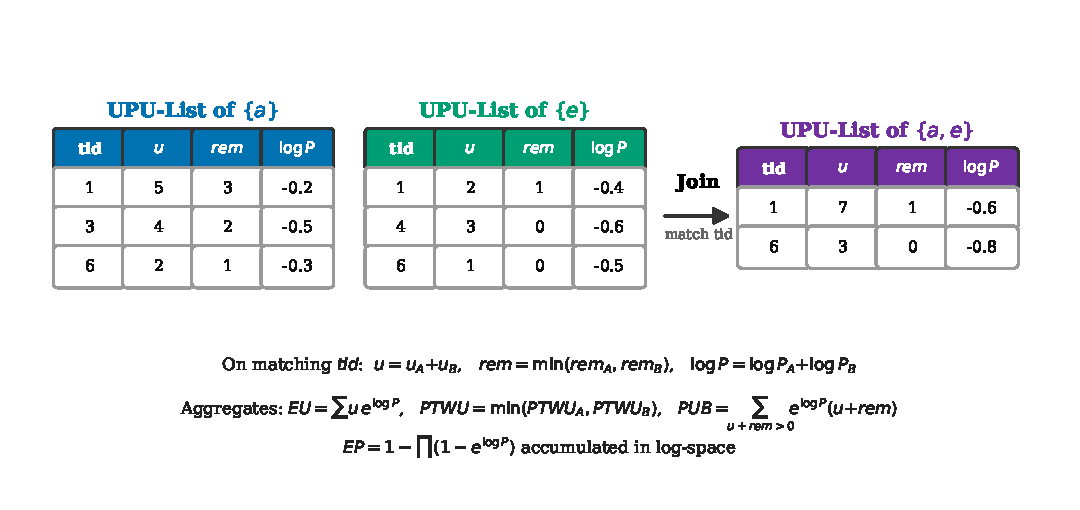
\includegraphics[width=\linewidth]{fig_upulist.pdf}
\caption{The UPU-List structure and the two-pointer \textsc{Join}. Entries sharing
a transaction id are merged, summing utility and log-probability and taking the
minimum remaining utility; the join also accumulates the cached aggregates
$\EU$, $\EP$, $\PTWU$ and $\PUB$.}\label{fig:upulist}
\end{figure}
\begin{gather}
\PTWU(\itemset)=\sum_{T\supseteq \itemset}\PTU(T), \qquad
\rem(\itemset,T)=\sum_{\substack{i\in T,\ i\succ \itemset,\ \pr(i)>0}}\pr(i)\qty(i,T), \label{eq:ptwurem}\\
\PUB(\itemset)=\sum_{\substack{T\supseteq \itemset:\ \uu(\itemset,T)+\rem(\itemset,T)>0}}\mathrm{P}(\itemset,T)\bigl(\uu(\itemset,T)+\rem(\itemset,T)\bigr). \label{eq:pub}
\end{gather}
An \emph{extension} of $\itemset$ is any $Z\supseteq \itemset$ whose extra items
follow $\itemset$ under $\prec$.

\begin{lemma}[$\EP$ anti-monotonicity]\label{lem:ep}
If $\itemset\subseteq Z$ then $\EP(Z)\le\EP(\itemset)$.
\end{lemma}
\begin{proof}
$\mathrm{P}(Z,T)\le\mathrm{P}(\itemset,T)$ as each $\prob(i,T)\in(0,1]$, so
$1-\mathrm{P}(Z,T)\ge1-\mathrm{P}(\itemset,T)$ for all $T$ and the product over
$T$ is no smaller for $Z$; hence $\EP(Z)\le\EP(\itemset)$.
\end{proof}

\begin{lemma}[$\PTWU$ bound]\label{lem:ptwu}
$\EU(Z)\le\PTWU(Z)\le\PTWU(\itemset)$ for any $\itemset\subseteq Z$.
\end{lemma}
\begin{proof}
For $T\supseteq Z$, $\uu(Z,T)\mathrm{P}(Z,T)\le\max\{\uu(Z,T),0\}\le\PTU(T)$:
if $\uu(Z,T)\ge0$ then multiplying by $\mathrm{P}(Z,T)\in(0,1]$ does not increase
it, otherwise the left side is negative; and the positive part of $\uu(Z,T)$ is
at most the positive utilities of $T$. Summing over $T\supseteq Z$ gives
$\EU(Z)\le\PTWU(Z)$. Since $\{T\supseteq Z\}\subseteq\{T\supseteq \itemset\}$ and
$\PTU\ge0$, $\PTWU(Z)\le\PTWU(\itemset)$.
\end{proof}

\begin{lemma}[$\PUB$ bound]\label{lem:pub}
For every extension $Z$ of $\itemset$, $\EU(Z)\le\PUB(\itemset)$.
\end{lemma}
\begin{proof}
For $T\supseteq Z$ the extra items of $Z$ lie in the $\prec$-suffix, so their
positive contribution is at most $\rem(\itemset,T)$ and
$\uu(Z,T)\le\uu(\itemset,T)+\rem(\itemset,T)$; also
$\mathrm{P}(Z,T)\le\mathrm{P}(\itemset,T)$ by Lemma~\ref{lem:ep}. Hence
$\uu(Z,T)\mathrm{P}(Z,T)\le\max\{0,\uu(\itemset,T)+\rem(\itemset,T)\}\,\mathrm{P}(\itemset,T)$.
Summing over $T\supseteq Z$ and dropping the non-positive terms gives
$\EU(Z)\le\PUB(\itemset)$.
\end{proof}

\begin{theorem}[Correctness]\label{thm:correct}
Pruning $\itemset$ when $\EP(\itemset)<\minprob$, $\PTWU(\itemset)<\tau$, or
$\PUB(\itemset)<\tau$---where $\tau$ is the current $K$-th largest admitted
$\EU$---never discards an itemset of an exact top-$K$ solution. Hence the search
is exact.
\end{theorem}
\begin{proof}
$\tau$ only increases and never exceeds the final $K$-th best $\EU$. By
Lemma~\ref{lem:ep} an itemset failing the $\EP$ test and all its extensions are
invalid. By Lemmas~\ref{lem:ptwu}--\ref{lem:pub}, $\PTWU(\itemset)<\tau$ or
$\PUB(\itemset)<\tau$ implies $\EU(Z)\le\tau$ for every extension $Z$, so none can
displace a current top-$K$ member. Thus only subtrees lying entirely below the
final threshold are pruned.
\end{proof}

\begin{remark}[Why sharing helps and why negatives matter]\label{rem:sharing}
Theorem~\ref{thm:correct} holds for any $\tau$ not exceeding the final $K$-th best
$\EU$. Raising $\tau$ earlier---as when many workers feed a shared
collector---prunes more without ever discarding a solution; a thread-local
threshold is simply a smaller, also-safe $\tau$ that prunes less. Negative items
depress $\EU$ and slow the ascent of $\tau$, which both reduces the benefit of
sharing and increases redundant parallel exploration.
\end{remark}

\subsection{Pattern Growth}\label{subsec:dfs}
Algorithm~\ref{alg:dfs} is the shared growth procedure; $\tau$ is read from a
top-$K$ collector holding the current $K$ highest-$\EU$ itemsets.

\begin{algorithm}[t]
\caption{\textsc{Grow}: depth-first pattern growth from a prefix}\label{alg:dfs}
\begin{algorithmic}[1]
\Require prefix $P$, start index $s$, ordered items $\sigma$, $1$-itemset lists $\mathcal{L}$, collector $C$, $\minprob$
\State $\tau \gets C.\textsc{threshold}()$
\If{$P.\PTWU < \tau$} \Return \EndIf
\For{$j \gets s$ \textbf{to} $|\sigma|-1$}
  \State $J \gets \textsc{Join}(P,\ \mathcal{L}[\sigma[j]],\ \tau)$
  \If{$J=\textsc{null}$ \textbf{or} $J.\EP<\minprob$ \textbf{or} $J.\PTWU<\tau$ \textbf{or} $J.\PUB<\tau$} \textbf{continue} \EndIf
  \If{$J.\EU \ge \tau$} $C.\textsc{tryCollect}(J)$ \EndIf
  \State \textsc{Grow}($J,\ j{+}1,\ \sigma,\ \mathcal{L},\ C,\ \minprob$)
\EndFor
\end{algorithmic}
\end{algorithm}

The growth procedure relies on two further operations: the list \textsc{Join}
(Algorithm~\ref{alg:join}), which merges a prefix with an extension item in one
linear pass while computing $\EU$, $\EP$, $\PTWU$ and $\PUB$; and
\textsc{TryCollect} (Algorithm~\ref{alg:collect}), the thread-safe admission of a
candidate into the shared top-$K$ heap. \textsc{TryCollect} uses a volatile
threshold for a lock-free fast reject and takes the lock only when a candidate
might actually be admitted; this is what lets the shared-threshold strategies
propagate $\tau$ cheaply across workers.

\begin{algorithm}[t]
\caption{\textsc{Join}: merge a prefix list with an extension-item list}\label{alg:join}
\begin{algorithmic}[1]
\Require prefix list $A$, extension list $B$ (item $e$), threshold $\tau$
\State $\rho \gets \min(A.\PTWU,\ B.\PTWU)$
\If{$\rho < \tau$} \Return \textsc{null} \EndIf \Comment{Tier 2, before the merge}
\State $eu \gets 0$;\ $ub \gets 0$;\ $\ell c \gets 0$;\ $L \gets$ empty list \Comment{$\ell c=\textstyle\sum\log(1-\mathrm P)$}
\State $i \gets 0$;\ $j \gets 0$
\While{$i<|A|$ \textbf{and} $j<|B|$}
  \If{$A.tid_i = B.tid_j$}
     \State $u \gets A.u_i + B.u_j$;\ \ $r \gets \min(A.r_i,B.r_j)$;\ \ $\ell p \gets A.\ell p_i + B.\ell p_j$
     \State append $(A.tid_i,\,u,\,r,\,\ell p)$ to $L$
     \State $eu \gets eu + u\cdot e^{\ell p}$
     \If{$u+r>0$} $ub \gets ub + e^{\ell p}(u+r)$ \EndIf
     \State $\ell c \gets \ell c + \log(1-e^{\ell p})$
     \State $i \gets i+1$;\ $j \gets j+1$
  \ElsIf{$A.tid_i < B.tid_j$} $i \gets i+1$
  \Else\ $j \gets j+1$
  \EndIf
\EndWhile
\If{$L$ is empty} \Return \textsc{null} \EndIf
\State \Return list for $A\cup\{e\}$ with $\EU{=}eu$, $\EP{=}1-e^{\ell c}$, $\PTWU{=}\rho$, $\PUB{=}ub$
\end{algorithmic}
\end{algorithm}

\begin{algorithm}[t]
\caption{\textsc{TryCollect}: admit a candidate into the shared top-$K$}\label{alg:collect}
\begin{algorithmic}[1]
\Require candidate $J$; min-heap $H$ ordered by $\EU$; size $K$; volatile threshold $\tau$
\If{$J.\EU < \tau$} \Return \EndIf \Comment{lock-free fast reject}
\State \textbf{acquire lock}
\If{$J.\EU \ge \tau$}
  \State $H.\textsc{push}(J)$
  \If{$|H| > K$} $H.\textsc{popMin}()$ \EndIf
  \State $\tau \gets (|H| < K)\ ?\ -\infty\ :\ H.\textsc{min}().\EU$
\EndIf
\State \textbf{release lock}
\end{algorithmic}
\end{algorithm}

\subsection{Five Parallelisation Strategies}\label{subsec:parallel}
The strategies span two axes: whether the admission threshold is \emph{shared},
and how prefix tasks are \emph{balanced} (Figure~\ref{fig:strategies}).

\begin{figure}[t]
\centering
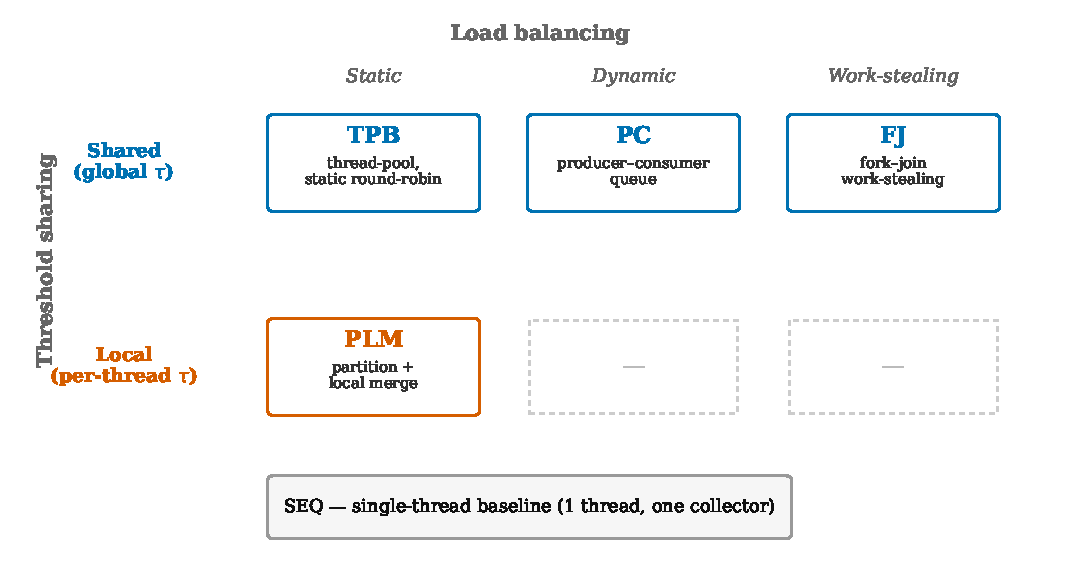
\includegraphics[width=\linewidth]{fig_strategies.pdf}
\caption{The shared-memory design space. The five strategies are placed by
whether they share the global admission threshold $\tau$ (rows) and how they
balance prefix tasks (columns). SEQ is the single-thread baseline.}\label{fig:strategies}
\end{figure}
\begin{itemize}
\item \textbf{SEQ} --- single thread over all $1$-itemset prefixes; the work and
time baseline.
\item \textbf{FJ} --- fork--join: prefixes are recursively split into balanced
batches on a work-stealing pool; one shared collector, so any worker's discovery
raises $\tau$ for all.
\item \textbf{TPB} --- thread-pool: prefixes assigned round-robin by $\PTWU$ rank
to a fixed pool; shared collector, static one-prefix tasks.
\item \textbf{PLM} --- partition--local merge: $\PTWU$-balanced blocks, each mined
into a \emph{thread-local} collector, merged at the end; no threshold sharing.
\item \textbf{PC} --- producer--consumer: a producer enqueues prefix tasks on a
bounded queue, consumers mine into a shared collector; dynamic scheduling.
\end{itemize}
By Remark~\ref{rem:sharing}, FJ, TPB and PC prune against the global $K$-th best,
whereas PLM prunes against weaker local thresholds. SEQ runs the prefixes of
Phase~3 in a single loop, and TPB submits one static \textsc{Grow} task per
prefix (in $\PTWU$ order) to a fixed pool that shares the collector; both are
straightforward and omitted. The three non-trivial schedulers are given in
Algorithms~\ref{alg:fj}--\ref{alg:pc}. FJ (Algorithm~\ref{alg:fj}) recursively
halves the prefix range on a work-stealing pool, balancing load dynamically while
sharing one collector. PLM (Algorithm~\ref{alg:plm}) gives each thread a
$\PTWU$-balanced block and its \emph{own} collector, merging them only at the end.
PC (Algorithm~\ref{alg:pc}) feeds prefixes through a bounded queue to consumer
threads that share the collector.

\begin{algorithm}[t]
\caption{\textsc{ForkJoinMine} (FJ): recursive prefix-batch scheduling}\label{alg:fj}
\begin{algorithmic}[1]
\Require prefix range $[lo,hi)$, ordered items $\sigma$, lists $\mathcal{L}$, \emph{shared} collector $C$, $\minprob$
\If{$hi - lo \le 1$}
  \For{$p \gets lo$ \textbf{to} $hi-1$}
     \State \textsc{Grow}($\mathcal{L}[\sigma[p]],\ p{+}1,\ \sigma,\ \mathcal{L},\ C,\ \minprob$)
  \EndFor
  \State \Return
\EndIf
\State $m \gets \lfloor (lo+hi)/2 \rfloor$
\State \textbf{fork} \textsc{ForkJoinMine}($[lo,m),\dots$) \Comment{stolen by an idle worker}
\State \textsc{ForkJoinMine}($[m,hi),\dots$) \Comment{run on the current worker}
\State \textbf{join} the forked task
\end{algorithmic}
\end{algorithm}

\begin{algorithm}[t]
\caption{\textsc{PartitionLocalMerge} (PLM): no threshold sharing}\label{alg:plm}
\begin{algorithmic}[1]
\Require ordered items $\sigma$, lists $\mathcal{L}$, size $K$, $\minprob$, threads $B$
\State partition $\{0,\dots,|\sigma|-1\}$ into $\PTWU$-balanced blocks $\Pi_1,\dots,\Pi_B$
\State create thread-local collectors $C_1,\dots,C_B$, each of size $K$
\For{$b \gets 1$ \textbf{to} $B$ \textbf{in parallel}}
  \For{$p \in \Pi_b$}
     \State \textsc{Grow}($\mathcal{L}[\sigma[p]],\ p{+}1,\ \sigma,\ \mathcal{L},\ C_b,\ \minprob$)
  \EndFor
\EndFor
\State $C \gets$ empty top-$K$;\quad \textbf{for} $b=1$ \textbf{to} $B$: $C.\textsc{merge}(C_b)$
\State \Return $C$
\end{algorithmic}
\end{algorithm}

\begin{algorithm}[t]
\caption{\textsc{ProducerConsumerMine} (PC): dynamic queue scheduling}\label{alg:pc}
\begin{algorithmic}[1]
\Require ordered items $\sigma$, lists $\mathcal{L}$, \emph{shared} collector $C$, $\minprob$, threads $N$
\State $Q \gets$ bounded blocking queue
\State \textbf{producer:} enqueue $0,\dots,|\sigma|-1$ into $Q$, then $N$ poison tokens
\For{each of $N$ consumers \textbf{in parallel}}
  \Loop
     \State $p \gets Q.\textsc{take}()$
     \If{$p$ is a poison token} \State \textbf{break} \EndIf
     \State \textsc{Grow}($\mathcal{L}[\sigma[p]],\ p{+}1,\ \sigma,\ \mathcal{L},\ C,\ \minprob$)
  \EndLoop
\EndFor
\end{algorithmic}
\end{algorithm}

\section{Experimental Setup}\label{sec:setup}
All algorithms are implemented in Java and share an identical mining core, so
performance differences isolate the parallelisation strategy.

\paragraph{Datasets and profit/probability assignment.}
We use four transactional benchmarks (Table~\ref{tab:datasets}): Chess and
Mushroom from the UCI Machine Learning Repository, the Retail dataset of a Belgian
retail store, and Liquor from the SPMF repository~\cite{fournierviger2014spmf}.
They span three orders of magnitude in density. Chess and Mushroom are dense,
fixed-length transactions; Retail and Liquor are sparse. To obtain a
positive--negative profit table, each item is assigned a profit and a fraction of
items is made negative, giving the negative fractions ($\%\mathrm{neg}$, $30$--$51\%$)
in Table~\ref{tab:datasets}; profit ranges and average positive/negative profits
are summarised in Table~\ref{tab:profits}. For Chess, Mushroom and Retail profits
are drawn at random; for Liquor each profit is the item's real average utility
(so positive profits can be large, up to $14{,}615$) and the $30\%$ of items with
the lowest utility are negated.

Regarding uncertainty, Chess, Mushroom and Retail are \emph{deterministic}: every
existence probability equals $1.0$, so they isolate the effects of density and of
positive/negative profits at scale (with $\minprob=0.7$ the $\EP$ filter is
inactive on these three). Liquor is the only dataset with \emph{genuine} per-item
existence probabilities, taken directly from the SPMF uncertain Liquor data; it is
therefore the case that exercises the full probabilistic setting.

\begin{table}[t]
\caption{Characteristics of the experimental datasets. $|T|$: transactions;
$|I|$: distinct items; avg$|t|$, max$|t|$: average and maximum transaction length;
Density $=$ avg$|t|/|I|$; $|I^-|$: negative-profit items; \%neg: their
fraction.}\label{tab:datasets}
\footnotesize\setlength{\tabcolsep}{4pt}
\begin{tabular}{@{}lrrrrrrrl@{}}
\toprule
Dataset & $|T|$ & $|I|$ & avg$|t|$ & max$|t|$ & Density & $|I^-|$ & \%neg & Source \\
\midrule
Chess    & 3{,}196  & 75      & 37.00 & 37 & 49.33\% & 38     & 50.7\% & UCI \\
Mushroom & 8{,}124  & 119     & 23.00 & 23 & 19.33\% & 45     & 37.8\% & UCI \\
Retail   & 88{,}162 & 16{,}470 & 10.31 & 76 & 0.063\% & 8{,}247 & 50.1\% & Belgian retail \\
Liquor   & 52{,}131 & 4{,}026 & 7.87  & 11 & 0.196\% & 1{,}207 & 30.0\% & SPMF (conv.) \\
\botrule
\end{tabular}
\end{table}

\begin{table}[t]
\caption{Profit-table statistics and the observed $\EU$ range of the top-$K$
results (over the swept $K$).}\label{tab:profits}
\footnotesize\setlength{\tabcolsep}{5pt}
\begin{tabular}{@{}lrrrr@{}}
\toprule
Dataset & Profit range & Avg.\ pos. & Avg.\ neg. & $\EU$ range of top-$K$ \\
\midrule
Chess    & $[-63.0,\,+48.0]$    & $+16.22$  & $-17.05$ & $[43{,}091,\ 151{,}130]$ \\
Mushroom & $[-60.0,\,+90.0]$    & $+18.41$  & $-17.38$ & $[61{,}761,\ 451{,}145]$ \\
Retail   & $[-130.0,\,+130.0]$  & $+17.26$  & $-17.17$ & $[3{,}348,\ 1{,}229{,}567]$ \\
Liquor   & $[-27.5,\,+14{,}615.0]$ & $+148.61$ & $-17.55$ & $[661,\ 560{,}291]$ \\
\botrule
\end{tabular}
\end{table}

\paragraph{Parameters.}
Because the appropriate $K$ differs by density, we sweep
$K\in\{10,20,30,40,50\}$ for Chess, $\{30,\dots,70\}$ for Mushroom,
$\{500,\dots,900\}$ for Retail, and $\{600,\dots,1000\}$ for Liquor;
$\minprob=0.7$ throughout. SEQ is the single-thread baseline and the parallel
strategies are run at $\{2,4,8\}$ threads.

\paragraph{Metrics and protocol.}
We report wall-clock time, speedup relative to SEQ, and a \emph{work ratio}: the
number of UPU-List joins performed by a strategy divided by that of SEQ at the
same $(K,\minprob)$. The work ratio separates algorithmic effects (how much of
the tree is explored, which threshold sharing changes) from hardware
parallelism. Experiments ran on an Intel Core i7-10700K (8 physical cores,
3.8\,GHz base) with 32\,GB RAM under Java~17; each configuration was executed
three times and the median is reported.

\section{Results}\label{sec:results}
Across all datasets and configurations every strategy returned exactly $K$
patterns identical to SEQ, consistent with Theorem~\ref{thm:correct}. We focus on
performance.

Table~\ref{tab:summary} reports speedup and work ratio at eight threads for the
largest $K$ of each dataset. Figure~\ref{fig:speedup} shows speedup versus $K$
(all $K$ values) at eight threads, and Figure~\ref{fig:workratio} shows the work
ratio versus $K$.

\begin{table}[t]
\caption{Speedup ($s$) and work ratio ($w$) at 8 threads, largest $K$ per
dataset. Work ratio $<1$ means a strategy performs less work than SEQ.}\label{tab:summary}
\begin{tabular}{@{}llrcccc@{}}
\toprule
Dataset & $K$ & SEQ (ms) & FJ ($s$/$w$) & TPB ($s$/$w$) & PC ($s$/$w$) & PLM ($s$/$w$) \\
\midrule
Chess    & 50   & 69509 & \textbf{27.5}/0.11 & 4.7/1.19 & 4.7/1.23 & 0.7/7.92 \\
Mushroom & 70   & 7841  & \textbf{10.0}/0.44 & 8.4/0.52 & 8.6/0.54 & 0.9/4.28 \\
Liquor   & 1000 & 8499  & 2.4/1.19 & 3.1/1.09 & \textbf{3.9}/1.07 & 2.4/1.66 \\
Retail   & 900  & 87442 & 2.2/1.18 & 2.7/1.11 & \textbf{3.4}/1.12 & 0.6/8.95 \\
\botrule
\end{tabular}
\end{table}

\begin{figure}[t]
\centering
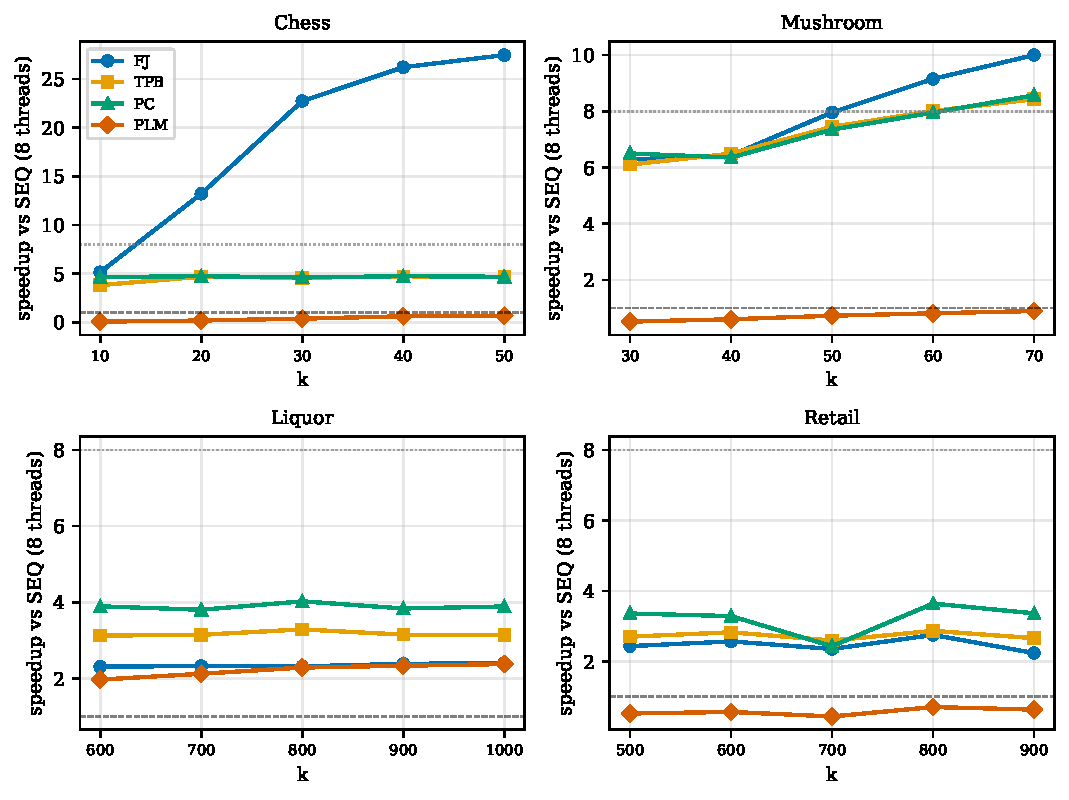
\includegraphics[width=\linewidth]{fig_speedup.pdf}
\caption{Speedup over SEQ versus $K$ at eight threads, for all $K$ values per
dataset. The dotted line marks eight-way (linear) speedup, the dashed line marks
parity with SEQ. FJ is super-linear on the dense datasets and its advantage grows
with $K$, but it is sub-linear on the sparse datasets, where PC scales best.}\label{fig:speedup}
\end{figure}

\begin{figure}[t]
\centering
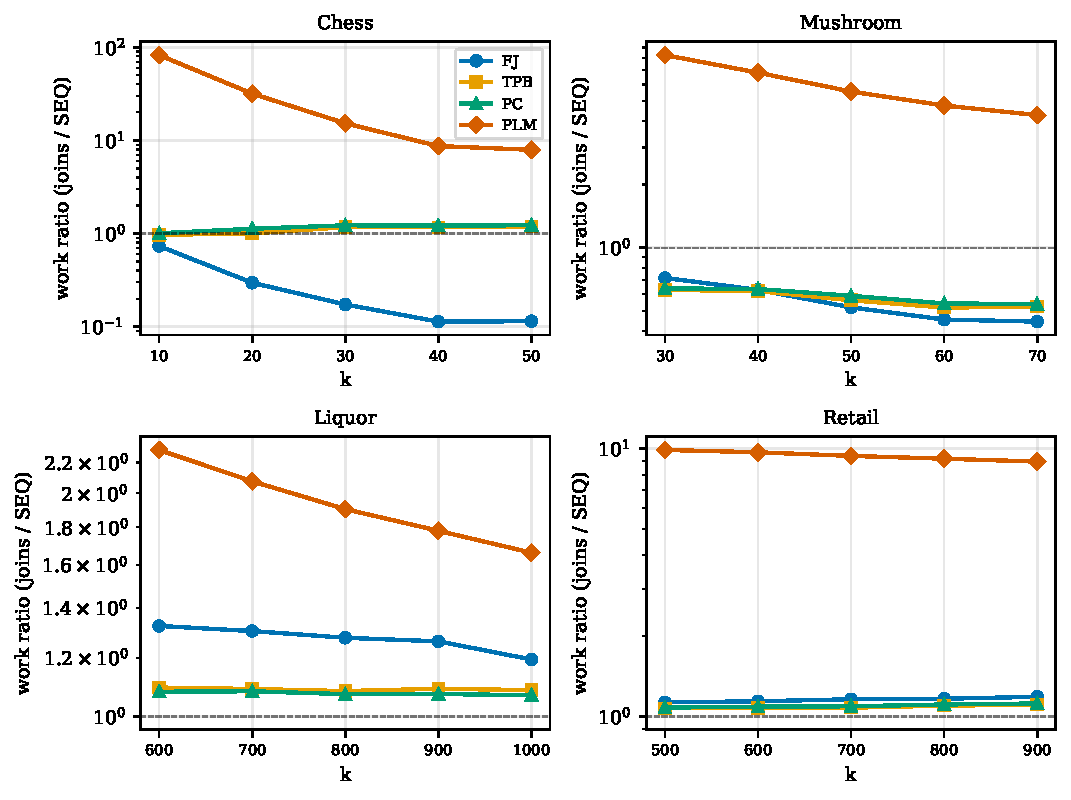
\includegraphics[width=\linewidth]{fig_workratio.pdf}
\caption{Work ratio (joins relative to SEQ, log scale) versus $K$ at eight
threads. Values below the dashed line ($=1$) mean less work than sequential. FJ
falls well below $1$ on dense data and rises above $1$ on sparse data; PLM is
always highest.}\label{fig:workratio}
\end{figure}

\paragraph{Dense data (Chess, Mushroom).} FJ's work ratio falls far below one
(to $0.11$ on Chess at $K=50$), i.e.\ cooperative threshold escalation prunes
roughly nine tenths of the sequential work. Combined with eight-way hardware
parallelism this yields \emph{super-linear} speedup, up to $27.5\times$ on eight
cores. TPB and PC also scale well ($\approx4.7\times$ on Chess,
$\approx8.5\times$ on Mushroom) but with higher work ratios than FJ
($\approx1.2$ on Chess, $\approx0.5$ on Mushroom), so they capture less of the
cooperative-pruning windfall.

\paragraph{Sparse data (Liquor, Retail).} Here FJ's work ratio exceeds one
($1.13$--$1.32$ over the sweep): the threshold rises slowly, so parallel branches
explore redundantly before pruning takes effect, and FJ's speedup collapses to
$\approx2.2$--$2.8\times$. The producer--consumer strategy PC is the most robust,
reaching $\approx3.4$--$4.0\times$ with a work ratio near one.

\paragraph{The non-sharing strategy.} PLM is the worst strategy in every regime,
and on Chess, Mushroom and Retail it runs \emph{slower than sequential}. Its work
ratio climbs steeply as $K$ shrinks: on Chess it reaches $\approx80\times$ the
sequential work at $K=10$ (Figure~\ref{fig:workratio}), so PLM can be more than
$10\times$ slower than SEQ (speedup as low as $0.07\times$); even at the largest
$K$ it still does $4$--$9\times$ the work (speedup $0.6$--$0.9\times$). The penalty
tracks how much pruning the shared threshold enables---largest where sharing
matters most, and smallest on Liquor, where PLM stays near a $2\times$ speedup.

\section{Discussion}\label{sec:discussion}
The work-ratio metric explains the whole spectrum. The benefit of sharing the
admission threshold is proportional to how quickly that threshold rises. On dense
data a few high-utility itemsets are found early, $\tau$ rises sharply, and a
strategy that propagates $\tau$ aggressively (FJ with work-stealing) converts
this into a large reduction in explored nodes---enough to make speedup
super-linear. On sparse data the utility landscape is flatter, $\tau$ rises
slowly, sharing buys little, and FJ's eager parallel splitting instead creates
redundant work; the more measured scheduling of PC then wins. PLM, which never
shares, forfeits whatever pruning the global threshold would have provided, so it
is worst everywhere and worst of all where that pruning is largest.

Two design lessons follow. First, no single strategy dominates: practitioners
should pick the strategy from the data regime, and the work ratio---measurable on
a small sample---predicts which regime applies. Second, super-linear speedup in
top-$K$ mining is an \emph{algorithmic} effect (cooperative pruning), not a
hardware one; reporting wall-clock speedup alone is misleading, and the work
ratio is needed to attribute it correctly.

On attribution: density, not the negative fraction. The regime tracks structural
density almost perfectly (Table~\ref{tab:datasets}): the two datasets where FJ
wins, Chess and Mushroom, have densities of $49.3\%$ and $19.3\%$, whereas the
two where PC wins, Retail and Liquor, are three orders of magnitude sparser
($0.063\%$ and $0.196\%$). The proportion of negative-profit items does
\emph{not} explain the split: Chess ($50.7\%$ negative) and Retail ($50.1\%$
negative) carry almost the same negative fraction yet fall in opposite regimes,
while Liquor has the fewest negatives ($30.0\%$) and still behaves like Retail.
Thus, although negative items slow the ascent of $\tau$ all else equal
(Remark~\ref{rem:sharing}), across these datasets it is density---through its
effect on how fast a few high-utility itemsets push $\tau$ up---that decides which
parallel strategy wins, not the negative fraction itself. Disentangling any
residual effect of the negative fraction would require holding density fixed
while varying it, which we leave to future work.

\paragraph{Threats to validity.} The profits and, for three datasets, the
existence probabilities are assigned rather than intrinsic, so they may not
reflect a specific application; in particular, only Liquor carries genuine
existence probabilities, while Chess, Mushroom and Retail are deterministic
($\EP=1$) and thus exercise the density and positive--negative dimensions but not
the probabilistic one. The study is single-machine and shared-memory; and PLM's
partitioning on one dataset (Retail) showed an unusually high work ratio that
merits closer inspection.

\section{Conclusion}\label{sec:conclusion}
We studied the shared-memory design space for mining top-$K$ probabilistic
positive--negative high-utility itemsets. A common UPU-List core with provably
sound three-tier pruning was instantiated under five parallel strategies, and a
work-ratio metric separated algorithmic pruning from hardware parallelism.
Experiments revealed a regime spectrum in which a work-stealing strategy attains
super-linear speedup on dense data but is beaten by a producer--consumer strategy
on sparse data, while a non-sharing strategy is uniformly worst. The regime is
governed by dataset density rather than by the negative-profit fraction. Future
work includes an adaptive scheduler that selects a strategy from a cheaply
measured work ratio, controlled experiments that isolate the effect of the
negative fraction at fixed density, and a distributed extension that approximates
global threshold sharing.

\section*{Declarations}

\bmhead{Funding}
\textcolor{gray}{[State funding, e.g.\ ``The authors received no specific
funding for this study,'' or list grant numbers.]}

\bmhead{Competing interests}
The authors declare no competing interests.

\bmhead{Ethics approval and consent to participate}
Not applicable. This study does not involve human participants, human data, or
animals.

\bmhead{Consent for publication}
Not applicable.

\bmhead{Data availability}
The Chess and Mushroom datasets are available from the UCI Machine Learning
Repository, and the Liquor dataset from the SPMF
repository~\cite{fournierviger2014spmf}; the Retail dataset is the publicly
available Belgian retail-store dataset. The profit tables and augmented
(positive--negative, and for Liquor uncertain) versions used here are available
from the authors on reasonable request. \textcolor{gray}{[Add a repository URL/DOI
if you deposit them.]}

\bmhead{Code availability}
The Java implementation of all five strategies and the shared mining core is
available from the authors on reasonable request. \textcolor{gray}{[Add the public
repository URL if applicable.]}

\bmhead{Author contributions}
H.~Vo and N.~Le contributed equally: they designed and implemented the
algorithms, ran the experiments, and drafted the manuscript. T.~Nguyen
supervised the work, contributed to the methodology, and revised the manuscript.
All authors read and approved the final version.

\begin{thebibliography}{10}
\providecommand{\doi}[1]{\url{https://doi.org/#1}}
\bibcommenthead

\bibitem[\protect\citeauthoryear{Liu and Qu}{2012}]{liu2012huiminer}
Liu M, Qu J.
\newblock Mining high utility itemsets without candidate generation.
\newblock In: Proc.\ 21st ACM Int.\ Conf.\ on Information and Knowledge
  Management (CIKM); 2012. p. 55--64.

\bibitem[\protect\citeauthoryear{Gan et~al.}{2021}]{gan2021survey}
Gan W, Lin JCW, Fournier-Viger P, Chao HC, Tseng VS, Yu PS.
\newblock A survey of utility-oriented pattern mining.
\newblock IEEE Transactions on Knowledge and Data Engineering.
  2021;33(4):1306--1327.

\bibitem[\protect\citeauthoryear{Wu et~al.}{2012}]{wu2012topk}
Wu CW, Shie BE, Tseng VS, Yu PS.
\newblock Mining top-K high utility itemsets.
\newblock In: Proc.\ 18th ACM SIGKDD Int.\ Conf.\ on Knowledge Discovery and
  Data Mining (KDD); 2012. p. 78--86.

\bibitem[\protect\citeauthoryear{Tseng et~al.}{2016}]{tseng2016topk}
Tseng VS, Wu CW, Fournier-Viger P, Yu PS.
\newblock Efficient Algorithms for Mining Top-K High Utility Itemsets.
\newblock IEEE Transactions on Knowledge and Data Engineering.
  2016;28(1):54--67.

\bibitem[\protect\citeauthoryear{Lin et~al.}{2016}]{lin2016phuim}
Lin JCW, Gan W, Fournier-Viger P, Hong TP, Tseng VS.
\newblock Efficient algorithms for mining high-utility itemsets in uncertain
  databases.
\newblock Knowledge-Based Systems. 2016;96:171--187.

\bibitem[\protect\citeauthoryear{Chu et~al.}{2009}]{chu2009huiniv}
Chu CJ, Tseng VS, Liang T.
\newblock An efficient algorithm for mining high utility itemsets with negative
  item values in large databases.
\newblock Applied Mathematics and Computation. 2009;215(2):767--778.

\bibitem[\protect\citeauthoryear{Lin et~al.}{2016}]{lin2016fhn}
Lin JCW, Fournier-Viger P, Gan W.
\newblock {FHN}: An efficient algorithm for mining high-utility itemsets with
  negative unit profits.
\newblock Knowledge-Based Systems. 2016;111:283--298.

\bibitem[\protect\citeauthoryear{Ryang and Yun}{2015}]{ryang2015rept}
Ryang H, Yun U.
\newblock Top-k high utility pattern mining with effective threshold raising
  strategies.
\newblock Knowledge-Based Systems. 2015;76:109--126.

\bibitem[\protect\citeauthoryear{Duong et~al.}{2016}]{duong2016khmc}
Duong QH, Liao B, Fournier-Viger P, Dam TL.
\newblock An efficient algorithm for mining the top-k high utility itemsets,
  using novel threshold raising and pruning strategies.
\newblock Knowledge-Based Systems. 2016;104:106--122.

\bibitem[\protect\citeauthoryear{Lin et~al.}{2017}]{lin2017muhui}
Lin JCW, Gan W, Fournier-Viger P, Hong TP, Tseng VS.
\newblock Efficiently mining uncertain high-utility itemsets.
\newblock Soft Computing. 2017;21(11):2801--2820.

\bibitem[\protect\citeauthoryear{Singh et~al.}{2018}]{singh2018negsurvey}
Singh K, Singh SS, Kumar A, Biswas B.
\newblock High utility itemsets mining with negative utility value: A survey.
\newblock Journal of Intelligent \& Fuzzy Systems. 2018;35(6):6551--6562.

\bibitem[\protect\citeauthoryear{Gan et~al.}{2020}]{gan2020tophui}
Gan W, Wan S, Chen J, Chen CM, Qiu L.
\newblock {TopHUI}: Top-k high-utility itemset mining with negative utility.
\newblock In: Proc.\ IEEE Int.\ Conf.\ on Big Data (Big Data). IEEE; 2020. p.
  5350--5359.

\bibitem[\protect\citeauthoryear{Lin et~al.}{2015}]{lin2015bigdata}
Lin YC, Wu CW, Tseng VS.
\newblock Mining high utility itemsets in big data.
\newblock In: Advances in Knowledge Discovery and Data Mining (PAKDD).
  Springer; 2015. p. 649--661.

\bibitem[\protect\citeauthoryear{Lin et~al.}{2019}]{lin2019pku}
Lin CH, Wu CW, Huang JT, Tseng VS.
\newblock Parallel Mining of Top-k High Utility Itemsets in Spark In-Memory
  Computing Architecture.
\newblock In: Advances in Knowledge Discovery and Data Mining (PAKDD).
  Springer; 2019. p. 234--246.

\bibitem[\protect\citeauthoryear{Sethi et~al.}{2018}]{sethi2018pfhm}
Sethi KK, Ramesh D, Edla DR.
\newblock {P-FHM+}: Parallel high utility itemset mining algorithm for big data
  processing.
\newblock Procedia Computer Science. 2018;132:918--927.

\bibitem[\protect\citeauthoryear{Fang et~al.}{2024}]{fang2024gpu}
Fang W, Jiang H, Lu H, Sun J, Wu X, Lin JCW.
\newblock {GPU}-based efficient parallel heuristic algorithm for high-utility
  itemset mining in large transaction datasets.
\newblock IEEE Transactions on Knowledge and Data Engineering.
  2024;36(2):652--667.

\bibitem[\protect\citeauthoryear{Fournier-Viger
  et~al.}{2014}]{fournierviger2014spmf}
Fournier-Viger P, Gomariz A, Gueniche T, Soltani A, Wu CW, Tseng VS.
\newblock {SPMF}: a Java open-source pattern mining library.
\newblock Journal of Machine Learning Research. 2014;15:3389--3393.

\end{thebibliography}


\end{document}